\documentclass{CPSReport}

\setminted[python3]{breaklines, framesep=2mm, fontsize=\footnotesize, numbersep=5pt}
\usemintedstyle{friendly}

%----------------------------------------------------------------------------------------
%	AUTHOR / TITLE INFORMATION
%----------------------------------------------------------------------------------------
\title{Assignment II: Statistics and Plotting + Digital Image Processing} % The article title

\author{
	\coursetitle{Introduction to Machine Learning Lab (190.013), SS2023}
	\authorstyle{Björn Ellensohn\textsuperscript{1}} % Authors
	\newline\newline % Space before institutions
	\textsuperscript{1}\textit{m01435615}, \textit{bjoern.ellensohn@stud.unileoben.ac.at}, \institution{Montanuniversität Leoben, Austria}\\ % Institution 1
	\submissiondate{\today} % Add a date here
}

%----------------------------------------------------------------------------------------
%	DOCUMENT
%----------------------------------------------------------------------------------------

\begin{document}

\maketitle % Print the title

\thispagestyle{firstpage} % Apply the page style for the first page (no headers and footers)

%----------------------------------------------------------------------------------------
%	ABSTRACT
%----------------------------------------------------------------------------------------

\lettrineabstract{This document guides through the process of solving Assignment 3.}

\section{Introduction}
The Task of 3rd assignment was coming up with an abstract class called \mintinline{python}{ContinuousDistribution} that provides the outline for two subclasses \mintinline{python}{GaussDistribution} and \mintinline{python}{BetaDistribution}.
Again, provided was a .csv file with a dataset.
The assignment is divided into three main parts and the bonus part.

\section{Part I - Abstract Class}
\subsection{Preparation}
When searching online for information on Python's abstract classes, you may come across the module known as \mintinline{python}{ABC}. This module includes a specific decorator, \mintinline{python}{@abstractmethod}, that can be used to define abstract methods. Essentially, this allows you to create a class that serves as a template or blueprint for other classes, without actually implementing the methods. To create a functional child class, you must define and implement the necessary methods there.

\subsection{Defining the Abstract Class}
The class \mintinline{python}{ContinuousDistribution} is created that provides the basic outline for the main classes of this exercise. The following functions should be inlcuded:
\begin{itemize}
    \item Data Import and Export using csv files.
    \item Computation of the mean based on the samples from the csv.
    \item Computation of the standard deviation based on the samples from the csv.
    \item Visualization of the distribution, the raw data or the generated samples.
    \item Generating/Drawing Samples from the distribution. 
\end{itemize}

So in the end, the abstract class \mintinline{python}{ContinuousDistribution} should look like this:

\begin{minted}{python3}
    import abc

    class ContinuousDistribution(metaclass=abc.ABCMeta):
    @abc.abstractmethod
    def import_data(self, file_path):
        pass

    @abc.abstractmethod
    def export_data(self, data, file_path):
        pass

    @abc.abstractmethod
    def compute_mean(self, data):
        pass

    @abc.abstractmethod
    def compute_standard_deviation(self, data):
        pass

    @abc.abstractmethod
    def visualize(self, data=None):
        pass

    @abc.abstractmethod
    def generate_samples(self, n_samples):
        pass
\end{minted}

\section{Part II - Plot and Sample Gaussian Distributions}
In the second part of this exercise, it is required to initiate a child class which is responsible for dealing with Gaussian distributions.

Explicitly, the following should be implemented:
\begin{itemize}
    \item Implement the functions defined in “ContinousDistribution”. 
    \item Implement a constructor that optionally takes the dimension of the multivariate distribution. 
    \item Implement a visualization for Multivariate Gaussians up to 3 dimensions.
    \item Find the empirical parameters of the distribution that created the samples in the ‘MGD.csv’ file.
    \item Plot the samples of the ‘MGD.csv’ file and the sample from the learned distribution in two subfigures.   
\end{itemize}

So the main goal of this class is to be able to compute the statistical parameters from a provided dataset and being able to sample a new dataset from this distribution. In the end, the datapoints should be plotted.

At first, let us declare how the Gaussian dsitribution is defined.
For all normal distributions, 68.2\% of the observations will appear within plus or minus one standard deviation of the mean; 95.4\% of the observations will fall within +/- two standard deviations; and 99.7\% within +/- three standard deviations. This fact is sometimes referred to as the "empirical rule," a heuristic that describes where most of the data in a normal distribution will appear.
This means that data falling outside of three standard deviations ("3-sigma") would signify rare occurrences.

In mathematical terms this is explained in \autoref{eq:1}.

\begin{equation} \label{eq:1}
    f(x)=\frac{1}{\sigma \sqrt{2\pi } } e^{-\frac{1}{2}(\frac{x-\mu}{\sigma})²}
\end{equation}

To sample from a multivariate Gaussian distribution, I will use a module called \mintinline{python}{multivariate_normal} from the \mintinline{python}{scipy} package.

The constructor of \mintinline{python}{GaussianDistribution} then looks like this:

\begin{minted}{python3}

class GaussDistribution(ContinuousDistribution):
    def __init__(self, dim=1):
        self.dim = dim
        self.mean = np.zeros(dim)
        self.covariance = np.eye(dim)
        self.data = pd.DataFrame()
        self.samples = None
\end{minted}

\autoref{fig:2} to \autoref{fig:4} are showing the end results.
In the appendix you will find the full code.

\begin{figure}[ht]
    \begin{center}
        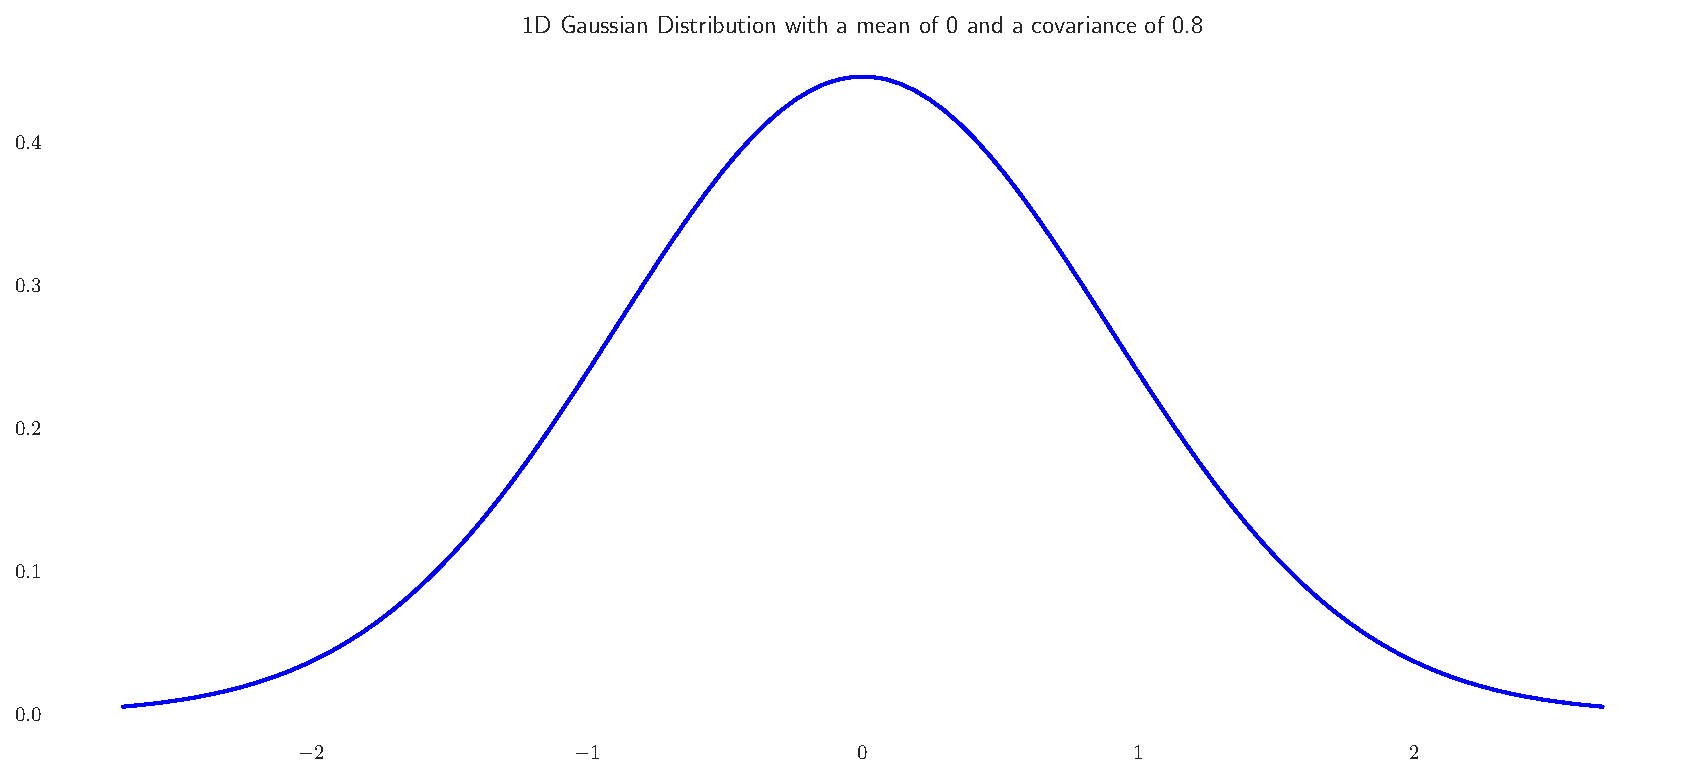
\includegraphics[width=1\linewidth]{../gaussian1D.pdf}
    \end{center}
    \caption{Plot of one dimensional Gaussian distribution.}
    \label{fig:2}
\end{figure}

\begin{figure}[ht]
    \begin{center}
        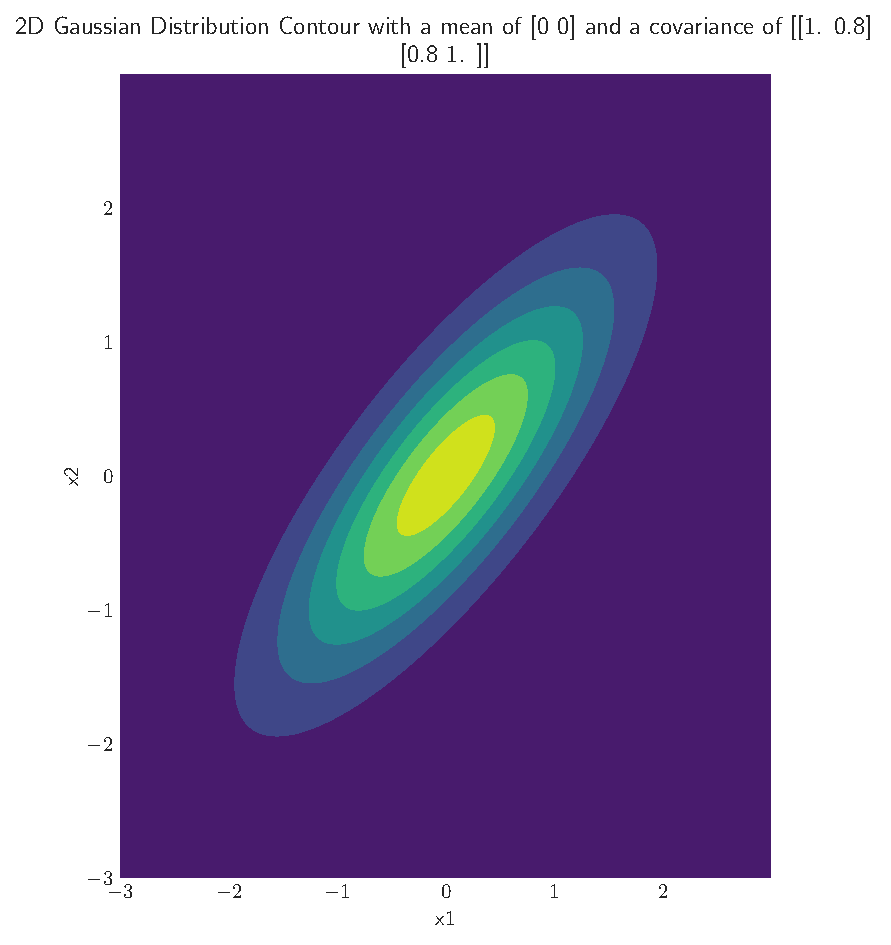
\includegraphics[width=1\linewidth]{../gaussian2D_contour.pdf}
    \end{center}
    \caption{Contour plot of two dimensional Gaussian distribution.}
    \label{fig:3}
\end{figure}

\begin{figure}[ht]
    \begin{center}
        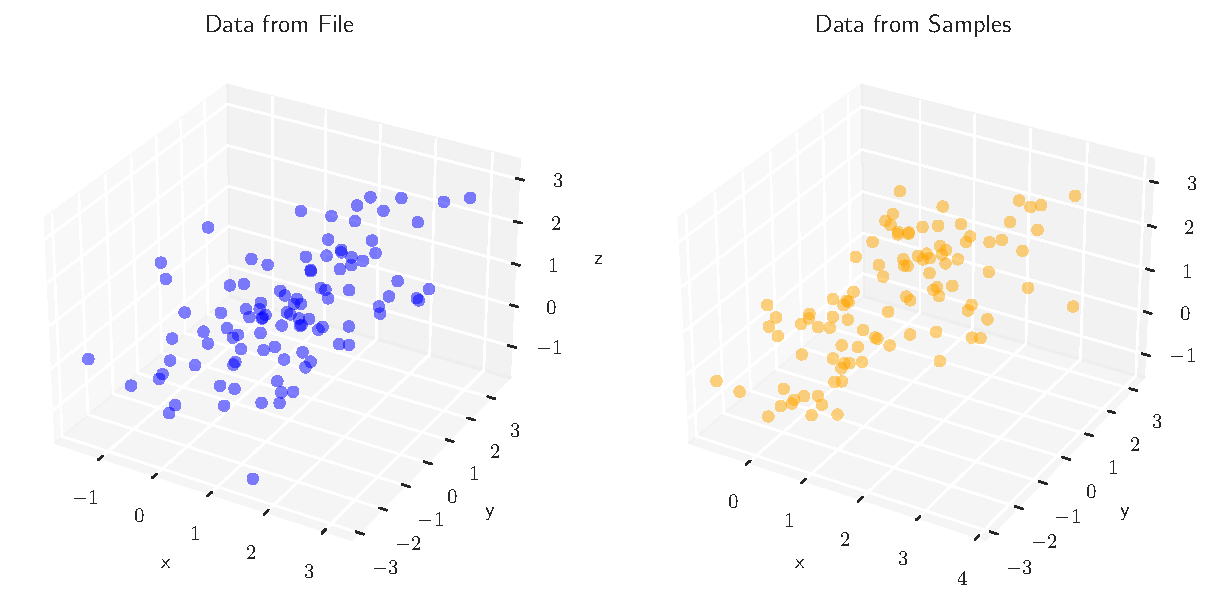
\includegraphics[width=1\linewidth]{../gaussian3D.pdf}
    \end{center}
    \caption{Plots of three dimensional Gaussian distribution.}
    \label{fig:4}
\end{figure}

\section{Part III - Plot and Sample Beta Distributions}
Next, a class \mintinline{python}{BetaDistribution} shouldbe inherited from the meta class. It should implement:

\begin{itemize}
    \item Generate beta distributed samples and plot the distribution giving the parameters a and b.
    \item The constructor should take the parameters a and b as arguments.
    \item A visualization for Beta distributions, including the mean and the standard deviation lines.
\end{itemize}

Again, there is a module in the \mintinline{python}{scipy} package that does the hard work here \mintinline{python}{beta}.
The constructor of \mintinline{python}{BetaDistribu
} then looks like this:

\begin{minted}{python3}
    class BetaDistribution(ContinuousDistribution):
    def __init__(self, a, b):
        self.a = a
        self.b = b
        self.data = None
\end{minted}

Provided is a plot showing the end results in \autoref{fig:1}.

\begin{figure}[ht]
    \begin{center}
        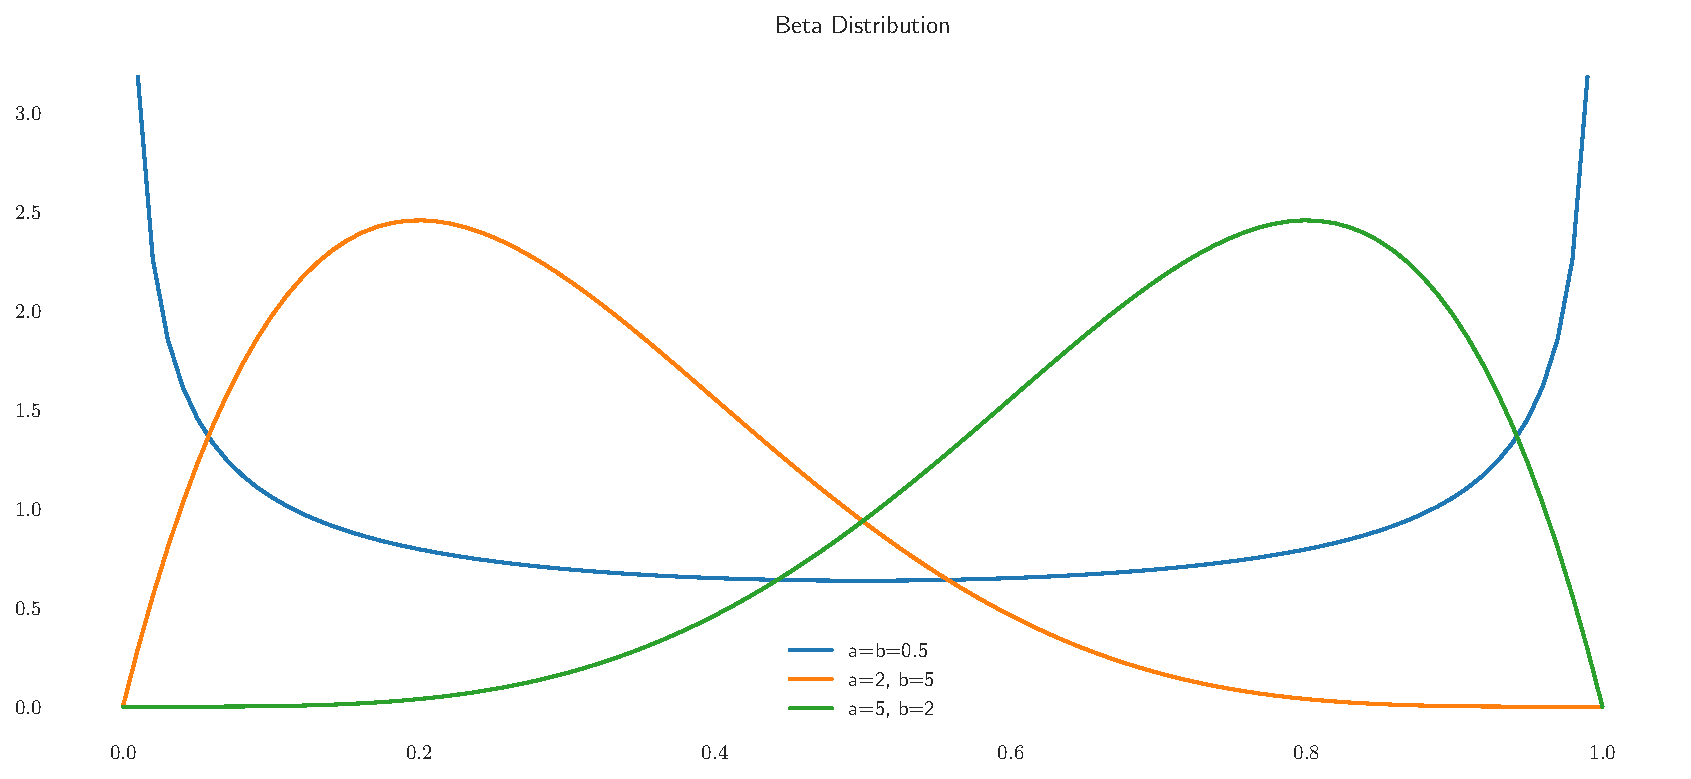
\includegraphics[width=1\linewidth]{../beta.pdf}
    \end{center}
    \caption{Plot of three different Beta Distributions.}
    \label{fig:1}
\end{figure}

\clearpage

\onecolumn
\section*{APPENDIX}\label{sec:appendix}

Ladies and Gentlemen, here I introduce the code. And figures.
\newline Questions to: bjoern.ellensohn@stud.unileoben.ac.at

% \subsection*{Code for Part I}
% \inputminted{python3}{code_example2a.py}

% \subsection*{Code for Part II}
% \inputminted{python3}{code_example2b.py}

% \subsection*{Code for Bonus Points}
% \inputminted{python3}{code_example_bonus.py}
% \newpage

\subsubsection*{Figures}

% \begin{figure}[ht]
%     \begin{center}
%         \includegraphics[width=.9\textwidth]{plots.pdf}
%     \end{center}
%     \caption{Three plots showing the capability of \mintinline{Python}{BasicStastistics}.}
%     \label{fig:1}
% \end{figure}

% \begin{figure}[ht]
%     \begin{center}
%         \includegraphics[width=.3\textwidth]{gaussian.pdf}
%     \end{center}
%     \caption{Applied Gaussian processing}
%     \label{fig:2}
% \end{figure}

% \begin{figure}[ht]
%     \begin{center}
%         \includegraphics[width=.3\textwidth]{laplacian.pdf}
%     \end{center}
%     \caption{Applied Laplacian processing}
%     \label{fig:3}
% \end{figure}

% \begin{figure}[ht]
%     \begin{center}
%         \includegraphics[width=.3\textwidth]{hand.pdf}
%     \end{center}
%     \caption{Raw Image}
%     \label{fig:4}
% \end{figure}

%----------------------------------------------------------------------------------------
\thispagestyle{lastpage}
\end{document}